\documentclass[10pt,twocolumn]{article}
\usepackage[margin=0.75in]{geometry}
\usepackage[T1]{fontenc}
\usepackage{lmodern}
\usepackage{microtype}
\usepackage{booktabs}
\usepackage{tabularx}
\usepackage{amsmath,amssymb}
\usepackage{graphicx}
\usepackage{xcolor}
\usepackage{tikz}
\usetikzlibrary{positioning,arrows.meta,calc}
\usepackage{url}
\usepackage[hidelinks]{hyperref}
\usepackage{cleveref}
\usepackage{placeins}

% Numbers that come from the analysis live in results.tex, which is regenerated from the run outputs
% (paper/make_results.py). Anything still pending prints as a red "TBD".
\newcommand{\tbd}[1]{\textcolor{red}{\textbf{TBD}\ifx&#1&\else~(#1)\fi}}
% Numbers for the paper. Pre-freeze values are filled in by hand from results/ and prereg/. The results texts were
% written by hand from results/ (main), results/heldout and results/audit after the runs finished on 2026-11-06;
% make_results.py only fills macros that still print TBD. Tables come from results_tables.tex (generated).
\newcommand{\resAbstractFinding}{that C verifies far more repairs than B for both primary models (Qwen3.5-2B: 27.7\%
of families vs 2.2\%; Qwen3.5-4B: 33.0\% vs 17.6\%; Holm $p<0.001$), and at least as many as BP (2B: +5.0
percentage points, $p_\text{Holm}=0.012$; 4B: a tie), while spending about 43\% fewer model tokens per verified
repair than BP and never asking the model for a proof. The held-out split replicates C over B and shows a C/BP tie
for both models. The gain comes from the automation more than from forbidding proofs: proof-writing agents that are
given the same portfolio first close most of the gap, and almost all of their successes are the portfolio's proofs,
not their own}

\newcommand{\resRQOneText}{\Cref{tab:rq1} gives the four confirmatory tests on the 106 \texttt{main} families that
carry a bug in the primary pool, and \cref{fig:rates} shows the rates for every condition.
\textbf{C vs B} is large and significant for both primary models: Qwen3.5-2B 27.7\% vs 2.2\% (+25.5\,pp, 95\% CI
[+18.2, +33.0]); Qwen3.5-4B 33.0\% vs 17.6\% (+15.4\,pp, [+9.4, +21.7]); $p_\text{Holm}<0.001$ for both. C
repairs 28 families that B never repairs for 2B (B: 0 that C misses), and 19 against 1 for 4B.
\textbf{C vs BP} is small. For 2B, C is ahead by +5.0\,pp ([+1.6, +8.8], $p_\text{Holm}=0.012$; 10 families only
by C, 2 only by BP). For 4B the two are tied: 33.0\% vs 32.7\% (+0.3\,pp, [$-$2.8, +3.5], $p_\text{Holm}=0.50$; 3
vs 2 families). The pre-freeze power analysis predicted exactly this: C vs BP had 0.71 power for 2B and 0.08 for
4B at the available families (\cref{tab:power}), so the 4B tie is reported as a tie, not as evidence of no
difference. Per-run rates (\cref{tab:rates}) and outcome labels (\cref{tab:outcomes}) tell the same story.
No run in any condition was \emph{verified but behaviourally wrong}, the outcome that would expose a weak
specification. Most failures in the proof-writing conditions are submissions rejected by the static checks;
they are mostly malformed rather than adversarial (lemmas placed in the helper region, a second definition of
the function, or proof text in the code region), and they are far rarer in C and C-plain (1,690 and 1,586
rejected attempts) than in A, B and BP (7,187, 5,662 and 5,764).}

\newcommand{\resCvsBPText}{The 4B tie stands as the result; four further facts say what it means. (i)~\emph{Power.} With 106 families, the pre-freeze simulation gave C vs BP a power of 0.08 for
4B (\cref{tab:power}): a difference of a few points could not have been detected, so the tie says ``no large
difference'', not ``equal''. (ii)~\emph{Where BP's successes come from.} BP is B with the portfolio run first. 180
of its 182 verified runs for 4B, and all 110 for 2B, were closed by the portfolio, not by the model's proof; the
proof-writing half of BP added two repairs out of 693 runs. BP is, in effect, C plus an expensive and almost
always failing proof attempt. (iii)~\emph{Cost.} For the same success rate, C spends 37k model tokens per verified
repair against BP's 65k (43\% fewer) and 68\,s of inference per run against 162\,s, because the model writes no
proof text; for 2B, 50k against 89k. (iv)~\emph{Integrity.} BP's submissions are rejected by the static checks
3.4 times as often as C's (5,764 against 1,690 rejected attempts), because proof text is where most malformed
submissions arise. The practical reading is that once automation is available, asking the model for a proof adds
cost and failure modes but no verified repairs.}

\newcommand{\resRQTwoText}{We classify each success as a \emph{revert} (identical to the reference, or within the
pre-registered distance of a reference that the portfolio proves), \emph{shaping} (the reference itself is
\emph{not} provable by the portfolio, so the verified code must have a different, automation-friendly shape) or
other. Shaping is common: 42 of 150 C successes for 2B and 81 of 191 for 4B are shaping, against 72 and 56
reverts. Where the reference is provable by the portfolio, C and BP both succeed on most runs (4B: 89.4\% and
91.1\%; B: 36.6\%). Where it is not, the rates fall for every condition, but C stays ahead of B (4B: 14.2\% vs
6.0\%; 2B: 7.4\% vs 0.0\%) and level with BP (12.3\%). Restricting the paired family-level test to the 85
\texttt{main} families whose reference the portfolio cannot prove, so that no success can be a plain revert
(\cref{tab:robust}, exploratory), C still beats B for every model (2B +10.6\,pp, 4B +7.8\,pp, Gemma +15.3\,pp;
$p\le0.002$), and is ahead of BP by +4.3 (2B, $p=0.035$), +1.2 (4B, $p=0.34$) and +7.1\,pp (Gemma, $p=0.055$). The
headline is therefore not carried by easy cases alone, although rates on these families are about half the
overall ones. Fifteen real before/after cases, each with the bug, the reference, C's verified code, the closing
tactic and what B did on the same run, are in \texttt{docs/code\_shapes.md}; \cref{fig:shape} shows one.
\textbf{Study S} asks the harder question directly:
starting from a \emph{correct} reference that the portfolio cannot prove, can a model re-shape it so that the
portfolio can? Rarely, and the structured hint does not help: 3.7\% (S) vs 4.1\% (S-plain) of runs for 2B and
12.7\% vs 12.7\% for 4B (family-level differences $-$0.4 and 0.0\,pp, $p=0.81$ and $0.60$). This suggests that
shaping in the repair setting happens mostly when fixing the bug and re-shaping the code coincide, not as a skill
of its own.}

\newcommand{\resRQThreeText}{The structured hint (witness, best unsolved goal, structural hint) does not beat a plain
retry. C vs C-plain: 2B 27.7\% vs 28.9\% ($-$1.3\,pp, [$-$3.8, +1.3], $p=0.89$), 4B 33.0\% vs 32.7\% (+0.3\,pp,
[$-$2.2, +2.8], $p=0.50$); 3 vs 3 and 2 vs 1 discordant families. C-plain is slightly cheaper (4B: 9.1k vs 10.3k
tokens and 58 vs 68\,s of inference per run). The benefit of C comes from the code-only contract and the
portfolio, not from the feedback text.}

\newcommand{\resRQFourText}{Recursion is the dominant blocker. Among the 184 eligible references (condition T), the
portfolio closes none of the 101 that use any recursion and 49.4\% of the rest; \texttt{let rec} (0 of 77) and
\texttt{match} (1.5\% vs 33.9\%) follow. The same holds for code the models write: among test-passing candidates
from the code-only conditions, 0.7\% of those with recursion are closed against 67.2\% without, 10.3\% with
\texttt{match} against 62.6\%, 29.7\% with \texttt{a[i]!} indexing against 58.7\%, and 23.7\% with
\texttt{Nat}/\texttt{Int} casts against 58.1\%. Folds and list combinators cost little ($-$4 and $-$10\,pp).
Verified repairs are closed mostly by the cheapest entries: for C, \texttt{simp} closes 146 of 399, \texttt{unfold}
+ \texttt{omega} 90, \texttt{simp\_all} 58, \texttt{simp}+\texttt{omega} 38 and \texttt{simp}+\texttt{grind} 36; the
induction entries never close a repair. Automation-friendly code, in practice, means non-recursive code built from
library combinators.}

\newcommand{\resRQFiveText}{\textbf{Cost.} C is the cheapest route to a verified repair (\cref{fig:costs}). For
Qwen3.5-4B, C spends 37k model tokens per verified repair, against 65k for BP and 165k for B, and 68\,s of
inference per run against 162\,s and 150\,s; for 2B, 50k against 89k (BP) and 1.5M (B). C spends more Lean time
per run (18\,s vs 6\,s for B with 4B) because the portfolio runs on every candidate. Truncating the generation
budget to 2 or 4 shows that C's lead is already present at $N=2$ (4B: 21.8\% vs 6.8\% of runs for B). Patch sizes
(normalised edit distance from the buggy start, successes only) are similar across conditions (4B: C 0.67, BP
0.52, B 0.77). \textbf{Scale.} Going from 2B to 4B helps B most (2.2\% $\to$ 17.6\%) and C least (27.7\% $\to$
33.0\%): the smaller model gains most from not writing proofs. \textbf{Second family.} Gemma-4-E4B (secondary)
repeats the pattern: C 30.2\% vs B 1.9\% (+28.3\,pp, $p<0.001$) and C vs BP 30.2\% vs 27.4\% (+2.8\,pp, [$-$3.8,
+9.4], $p=0.29$). \textbf{Proof specialist.} Goedel-Code-Prover-8B, run as a reference in A and B only, verifies
16.5\% and 20.8\% of runs, below Qwen3.5-4B in C (27.6\%), which has half the parameters and no proof training.
\textbf{Energy} (estimate, deviation D-4; \cref{tab:energy}). The study's energy counter read the wrong GPU, so
we calibrated joules per prompt and completion token for each model on our slice after the study. Each model was
replayed on prompts it had received, at the study's serving settings. C is also the most energy-efficient
condition: for Qwen3.5-4B it uses 2.6\,kJ per verified repair [2.4, 2.9], against 5.9\,kJ for BP and 13.4\,kJ for
B; for 2B, 2.0\,kJ against 3.6\,kJ and 56\,kJ; for Gemma, 2.6\,kJ against 8.8\,kJ and 232\,kJ. These are 0.4--0.5\,g of CO$_2$
per repair in C. The held-out split gives the same ordering (4B: 3.2, 7.4 and 24\,kJ). C's extra Lean time costs
less than the model tokens it saves. All study runs together used an estimated 3.1\,kWh (2.3\,kg CO$_2$). Running two
jobs side by side may raise absolute figures by up to about 1.6 times, but equally for every condition.}

\newcommand{\resSecondaryText}{\textbf{B without automation.} Many of B's own proofs are a single automation call.
Counting those as failures (B\_noauto) lowers B from 17.6\% to 12.3\% for 4B (C vs B\_noauto +20.8\,pp); for 2B,
B falls to 0.9\%. \textbf{Bhammer}, which tells B the portfolio's tactics in the prompt, helps B a little (4B:
24.2\% vs 17.6\%, +6.6\,pp, [+1.3, +11.9], $p=0.011$; 2B: 5.3\% vs 2.2\%, $p=0.057$) but stays below C (4B:
$-$8.8\,pp, $p=0.001$; 2B: $-$22.3\,pp, $p<0.001$); 95 of its 131 successes for 4B are automation-only proofs. Knowing
the tactics is not the same as having them run. \textbf{B$\to$C cross-evaluation.} We re-verified every B attempt
whose code compiled but whose proof failed through C's code-only pipeline. C's pipeline would have verified
30.8\% of these attempts for 4B (797 of 2,588), 34.0\% for 2B and 40.7\% for Gemma, and would have rescued 17.3\%,
16.8\% and 23.1\% of B's failed runs. None of these candidates passed the proof but failed the tests, so the
cross-evaluation found no weak specification. In B, the code was often right and the proof was the bottleneck.
\textbf{Natural bugs only.} Natural bugs cover only 33 \texttt{main} families, which is why the pre-registered
fallback pool applies. On those families alone (\cref{tab:robust}, exploratory), C beats B for every model (2B
14.1\% vs 0.0\%, $p=0.031$; 4B 18.2\% vs 0.0\%, $p=0.008$; Gemma 18.2\% vs 0.0\%, $p=0.016$), and C is ahead of BP
by 5--9\,pp without significance ($p$ from 0.06 to 0.13). Mutants alone reproduce the pooled results. Natural bugs
are harder for every condition, and the small pool limits what can be said about them beyond the direction.
\textbf{Re-verification.} \resReverifyText
\textbf{Audit.} The 10\% stratified audit plus every flagged success (333 runs, 126 distinct programs) found no
specification gaming in an automated pre-screen; the human audit is pending (deviation D-3). 27 runs decide the
postcondition proposition directly or carry dead code, and are reported as unnatural but correct. The spec-copying
flag fired on 239 of the audited runs, all of which restate an exact, executable postcondition.}

\newcommand{\resHeldoutText}{The held-out split (46 families with a bug in the primary pool) was run once and
analysed separately (\cref{tab:heldout}). C vs B replicates for both models: 2B 20.3\% vs 1.4\% (+18.8\,pp,
[+9.4, +29.0]), 4B 29.7\% vs 10.1\% (+19.6\,pp, [+10.1, +30.4]); $p_\text{Holm}=0.001$ for both. C vs BP is a tie for
both models (20.3\% vs 20.3\% and 29.7\% vs 29.7\%; $p_\text{Holm}=1.00$), so the 2B advantage of C over BP on
\texttt{main} does not replicate. No condition repaired any of the 10 held-out families with natural bugs.}

\newcommand{\resConclusionText}{Across 12,249 study runs on one GPU slice, letting automation carry the proof is the
most effective and cheapest way for small models to produce end-to-end verified repairs. C beats proof writing
(B) decisively, on \texttt{main} and on the held-out split, for two Qwen sizes and for Gemma. Against a
proof-writing agent that gets the same automation first (BP), C ties or wins narrowly, and the narrow win does not
replicate on held-out. It is clearly cheaper: about 43\% fewer tokens per verified repair and less than half the
inference time with 4B (and, by a post-hoc estimate, less than half the energy). The structured hint adds nothing
over a plain retry; recursion, \texttt{match} and array
indexing are what defeat the automation; and models rarely re-shape correct but unprovable code. The practical
lesson is to give small models a fixed automation portfolio and ask them only for code. Further gains will come
from widening what automation can prove, especially recursion, rather than from better feedback text.}

% from results/reverify/summary.md (scripts/reverify.py, 2026-11-14)
\newcommand{\resReverifyText}{After the study, every one of the 1,858 logged successes (all study folders) was given
again to the trusted judge from its logged code and proof, with the cache disabled and on a different machine and
operating system (a Windows laptop, same Lean and Mathlib). All 1,858 re-verify, each with the same proof source and
the same closing portfolio entry as logged (D-7). The verdicts therefore do not rest on the logs alone.}

\newcommand{\resFreezeDigest}{\texttt{3f2744e1\ldots}, 19 files, 2026-11-05}
\newcommand{\resTCoverage}{22.3\%: basic 35.6\%, advanced 5.0\%}
\newcommand{\resNaturalFamilies}{33}
\newcommand{\resPowerTable}{%
\begin{tabular}{@{}llrrr@{}}
\toprule
Comparison & Model & Point & Pessimistic & Families needed \\
\midrule
C vs B  & Qwen3.5-2B & 1.000 & 0.662 & 34 \\
C vs B  & Qwen3.5-4B & 0.996 & 0.128 & 57 \\
C vs BP & Qwen3.5-2B & 0.706 & 0.000 & 136 \\
C vs BP & Qwen3.5-4B & 0.082 & 0.000 & not reachable \\
\bottomrule
\end{tabular}}


\title{Prove Less, Repair Better: Automation-Friendly Program Repair\\for Small Models in Lean~4}
\author{Inesh Dheer \and Poojitha J \and Gracy Garg\\
\small Agents of Ultron --- Agentic Software Engineering (CS6.403), IIIT Hyderabad}
\date{}

\begin{document}
\maketitle

\begin{abstract}
Small, locally runnable language models rarely write valid Lean~4 proofs, yet they often write correct code.
We test whether they produce more \emph{end-to-end verified} repairs when they change only the implementation,
shaping it so that a fixed, pre-registered portfolio of Lean automation proves the unchanged specification
(condition C), than when they write the proofs themselves (B), or write proofs after the same automation has
already been tried (BP). On repair tasks derived from VERINA, with natural bugs from other models and
controlled mutants, budget-matched agents, hidden tests whose preconditions are proved in Lean, and a
pre-registered analysis with the task family as the unit, we find \resAbstractFinding.
We also measure \emph{why}: how often successes re-shape code for automation rather than revert the bug,
whether models can re-shape correct but unprovable code, and which code shapes automation proves.
Every step, from building the dataset to the final analysis, ran on one 48\,GB MIG slice of an NVIDIA RTX PRO
6000 Blackwell GPU, with 4-bit models.
\end{abstract}

\section{Introduction}
Proof generation is the bottleneck of verified code generation. On VERINA~\cite{verina}, the best model in the
published evaluation reached 72.6\% code correctness but only 4.9\% proof success. Small models, the ones
developers can run privately and cheaply, are weaker still. Lean~4, however, ships strong automation
(\texttt{simp}, \texttt{omega}, \texttt{decide}, \texttt{aesop}, \texttt{grind}) that closes many obligations
without hand-written tactics, \emph{provided the code has a suitable shape}.

We therefore move the proof burden from the model to the shape of the code. In condition C the model edits
only the implementation, and a fixed, pre-registered tactic portfolio must prove the unchanged contract. The
model never writes a tactic. We compare C against budget-matched proof-writing agents: B, which repairs code
and proof from Lean feedback; BP, which gets the same portfolio first and writes a proof only if it fails;
and A, a single-shot baseline.

\paragraph{Research questions.}
\textbf{RQ1} (confirmatory): at matched budget, does C reach a higher verified-repair rate than B and BP?
\textbf{RQ2} (mechanism): do successes come from re-shaping code for automation or from reverting the bug, and
can models re-shape correct but unprovable code (S vs S-plain)?
\textbf{RQ3} (feedback): does C's structured hint beat a plain retry (C vs C-plain)?
\textbf{RQ4} (code shapes): which implementation features predict that automation succeeds?
\textbf{RQ5} (costs and scale): tokens, inference time, Lean time, patch size and integrity flags; 2B vs 4B;
Qwen vs Gemma; a proof-specialist reference.

\paragraph{Contributions.}
(i)~A budget-matched comparison of code-only repair against proof-writing repair for small models, with a
B+P control that separates ``do not write proofs'' from ``automation exists'';
(ii)~a mechanism analysis (shaping vs reverting, study S, and a code-shape catalogue);
(iii)~a buggy-VERINA dataset with natural and mutant bugs and hidden tests with Lean-proved preconditions;
(iv)~a fully pre-registered protocol, with a frozen configuration hash and a public deviation log.
We do not claim novelty for compiler feedback, structured repair messages, automated tactics or code
restructuring in isolation.

\section{Related Work}
\textbf{Proof repair from compiler feedback.} APRIL trains models to repair Lean proofs from compiler errors and
goal states~\cite{april}; APOLLO combines Lean diagnostics, decomposition and automated solvers~\cite{apollo}.
Both repair the \emph{proof}; we leave the proof to fixed automation and repair the \emph{code}.
\textbf{Proof optimisation and joint planning.} ImProver and Lean Refactor rewrite existing
proofs~\cite{improver,leanrefactor}; P$^3$ plans programs and proofs jointly~\cite{p3}; Vero evaluates frontier
agents building verified repositories~\cite{vero}.
\textbf{Restructuring code for verification.} Dissect-and-Restore transiently refactors Dafny code for
SMT-based verification~\cite{dissect}, and DafnyFix repairs Dafny implementations with single
transformations~\cite{dafnyfix}. Neither uses small models or Lean automation.
\textbf{Verifier scaffolds and feedback.} A Lean verifier-guided scaffold documents specification hacking under
verifier rewards~\cite{mitthesis}; FeedbackEval and related work compare feedback types for LLM
repair~\cite{feedbackeval,propfeedback,symbolicfeedback}.
\textbf{Benchmarks and their defects.} VERINA~\cite{verina} and CLEVER~\cite{clever} pair specifications with
implementations. Two audits report VERINA specification issues~\cite{multimodalverifier,isomorphism}; all of
them were fixed upstream before our pinned commit (\cref{sec:prereg}).

\section{Method}
% Method overview: from a VERINA task to a verdict. Fixed coordinates so no edge crosses a box.
\begin{figure*}[t]
\centering
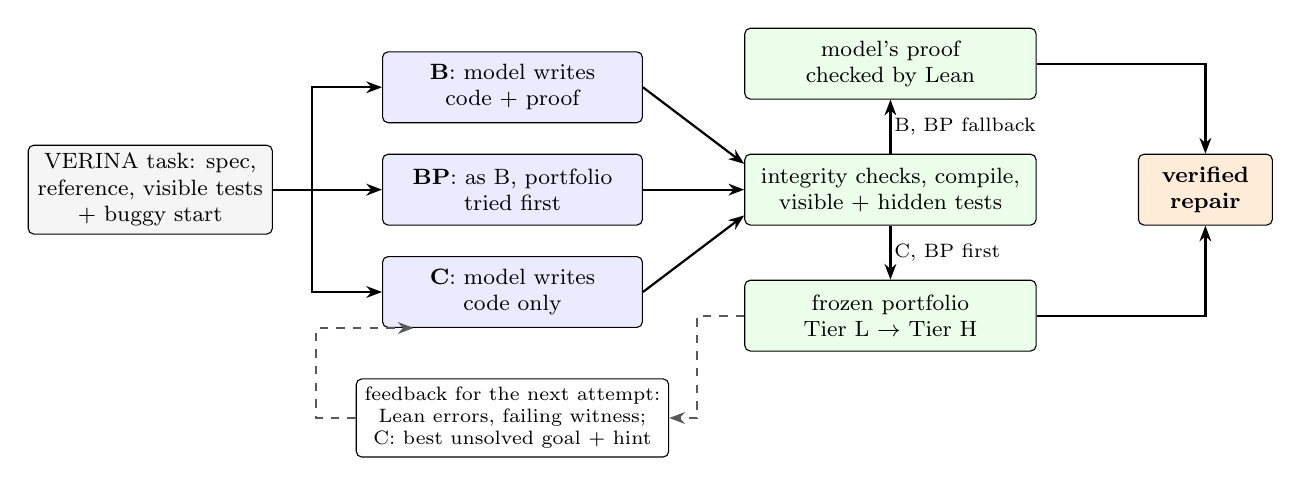
\begin{tikzpicture}[
  box/.style={draw, rounded corners=2pt, align=center, font=\footnotesize, minimum height=9mm, inner sep=3pt},
  data/.style={box, fill=gray!8, minimum width=31mm},
  model/.style={box, fill=blue!8, minimum width=33mm},
  lean/.style={box, fill=green!8, minimum width=37mm},
  verdict/.style={box, fill=orange!15, font=\footnotesize\bfseries, minimum width=17mm},
  arr/.style={-{Stealth[length=2mm]}, thick},
  fb/.style={-{Stealth[length=2mm]}, thick, dashed, gray!70!black},
  lab/.style={font=\scriptsize, fill=white, inner sep=1pt}]
\node[data]    (in)     at (0, 0)      {VERINA task: spec,\\reference, visible tests\\+ buggy start};
\node[model]   (B)      at (4.6, 1.3)  {\textbf{B}: model writes\\code + proof};
\node[model]   (BP)     at (4.6, 0)    {\textbf{BP}: as B, portfolio\\tried first};
\node[model]   (C)      at (4.6, -1.3) {\textbf{C}: model writes\\code only};
\node[lean]    (gate)   at (9.4, 0)    {integrity checks, compile,\\visible + hidden tests};
\node[lean]    (mp)     at (9.4, 1.6)  {model's proof\\checked by Lean};
\node[lean]    (port)   at (9.4, -1.6) {frozen portfolio\\Tier L $\to$ Tier H};
\node[verdict] (ok)     at (13.4, 0)   {verified\\repair};
\node[box, font=\scriptsize, minimum width=33mm] (fbk) at (4.6, -2.9)
  {feedback for the next attempt:\\Lean errors, failing witness;\\C: best unsolved goal + hint};
\draw[arr] (in.east) -- ++(0.5,0) |- (B.west);
\draw[arr] (in.east) -- (BP.west);
\draw[arr] (in.east) -- ++(0.5,0) |- (C.west);
\draw[arr] (B.east) -- (gate.170);
\draw[arr] (BP.east) -- (gate.west);
\draw[arr] (C.east) -- (gate.190);
\draw[arr] (gate.north) -- node[lab, right]{B, BP fallback} (mp.south);
\draw[arr] (gate.south) -- node[lab, right]{C, BP first} (port.north);
\draw[arr] (mp.east) -| (ok.north);
\draw[arr] (port.east) -| (ok.south);
\draw[fb] (port.west) -- ++(-0.6,0) |- (fbk.east);
\draw[fb] (fbk.west) -- ++(-0.5,0) |- (C.200);
\end{tikzpicture}
\caption{Method. Every condition gets the same buggy start, the same visible information and the same budget
(8 generations, 48k tokens, 600\,s of inference). A candidate must pass integrity checks, compile and pass every
visible and hidden test before any proof is tried; hidden tests are never shown to the model. In B the model's own proof must check; in C the model writes
no proof and a frozen two-tier portfolio of Lean automation must prove the unchanged specification; BP tries the
portfolio first and falls back to the model's proof. A failed attempt returns feedback for the next one (dashed),
in every condition except the single-shot baseline A.}
\label{fig:pipeline}
\end{figure*}

\subsection{Tasks and bugs}
VERINA has 189 Lean~4 tasks (pinned commit \texttt{66b3ce5}). A task is eligible if its reference compiles and
passes its tests; a human proof is \emph{not} required (only 46 of 189 ship one). Five tasks are excluded
(four known defects and one with unrenderable tests), leaving 184 eligible: 104 basic and 80 advanced.
Families are the statistical unit and are split at family level into pilot (20), main (114) and held-out (50).

\emph{Natural bugs} are zero-shot implementations by Qwen3.5-0.8B and Qwen3.5-9B, which never act as
repairers: at most four samples per generator and family, kept if they compile and fail at least one test.
\emph{Mutants} apply arithmetic, relational, boolean, constant, condition-negation, branch-swap, off-by-one and
argument-swap operators, kept if they compile and fail a test, at most two per family. The pre-registered pool
rule uses natural bugs if at least 60 \texttt{main} families carry one, and natural $\cup$ mutant otherwise.
Natural bugs cover \resNaturalFamilies{} of 114 \texttt{main} families, so the fallback pool applies; mutants are also reported
separately. \emph{Shaping instances} for study S are correct references that the portfolio alone cannot prove.

\emph{Hidden tests} are generated inputs whose precondition is \emph{proved in Lean}, with expected outputs from
the reference (30 per family). They are never shown to a model; failures are reported only as a count.

\subsection{Conditions}
\Cref{tab:conditions} lists the conditions. All share the same models, buggy starts, turn-0 information and
budget per (instance, condition, model, seed): at most 8 generations, 48k tokens and 600\,s of inference,
whichever binds first, with at most 1,536 completion tokens per generation. C and C-plain sample two
candidates per feedback round. Decoding uses temperature 0.7, top-$p$ 0.95, hidden reasoning disabled, and
seeds 11, 23 and 37.

\begin{table*}[t]
\centering\small
\caption{Conditions. The proof source is the only allowed one; everything else is shared.}
\label{tab:conditions}
\begin{tabularx}{\textwidth}{@{}l>{\raggedright\arraybackslash}X>{\raggedright\arraybackslash}X>{\raggedright\arraybackslash}X@{}}
\toprule
ID & Model writes & Proof from & Feedback \\
\midrule
T & --- & portfolio & --- \\
A & code + proof & model & none ($N$ samples) \\
B & code + proof & model & Lean errors, witness, proof errors \\
BP & code + proof & portfolio, else model & as B \\
\textbf{C} & code only & portfolio & witness, best unsolved goal, structural hint \\
C-plain & code only & portfolio & generic retry \\
S / S-plain & code, from a correct ref. & portfolio & as C / as C-plain \\
Bhammer$^\dagger$ & code + proof; prompt lists portfolio & model & as B \\
\bottomrule
\end{tabularx}\\[2pt]
\footnotesize $^\dagger$Exploratory, pre-registered to run unconditionally; never pooled with B.
\end{table*}

\subsection{Verification and the portfolio}
Verification uses Lean~4.24.0 with the whole of Mathlib v4.24.0, loaded once per worker in our own
verification server. A candidate is a \emph{verified repair} only if it compiles, passes all visible and hidden
tests, is proved by the allowed source, uses no axioms beyond \texttt{propext}, \texttt{Classical.choice} and
\texttt{Quot.sound}, leaves the locked regions (specification, theorem statement, tests) unchanged, and passes
static integrity checks. These reject \texttt{sorry}, \texttt{admit}, new axioms, \texttt{native\_decide},
\texttt{implemented\_by}, \texttt{unsafe}, \texttt{set\_option}, macros, attributes, redefinitions of locked
names, and any proof text in code-only conditions. Spec-copying, constant bodies, hard-coded tests and
\texttt{choice} are flagged for audit.

The portfolio is frozen. It runs in a fixed order and stops early: Tier~L (50k heartbeats) holds
\texttt{decide}, \texttt{simp}, \texttt{simp\_all}, and combinations with \texttt{omega} and \texttt{split};
Tier~H (200k heartbeats) holds \texttt{grind}, \texttt{aesop}, and functional or structural induction closed by
\texttt{simp\_all} or \texttt{grind}. Heartbeats are the tactic budget; wall-clock guards only stop hangs.
Infrastructure failures never charge the model's budget.

\subsection{Analysis}
\label{sec:analysis}
The family score is the mean over seeds of ``any instance of the family solved''. RQ1 uses a one-sided paired
sign-flip permutation test on family scores (100,000 permutations), Holm-corrected over the four primary tests
(C vs B and C vs BP, for each primary model), plus exact McNemar on majority-solved families, 95\%
family-cluster bootstrap intervals (10,000 resamples) and Cohen's $h$. Secondary analyses are never pooled with
the primary ones: \textbf{B\_noauto} counts B's successes whose proof is a single call to automation as
failures; \textbf{Bhammer} is compared with B and C; and the \textbf{B$\to$C cross-evaluation} re-checks every
B attempt whose code compiled but whose proof failed through C's code-only pipeline. The held-out split is
analysed once and separately, as a replication.

\section{Pre-registration, Freeze and Deviations}
\label{sec:prereg}
\textbf{One environment for everything.} Every step of the study ran on one 48\,GB MIG slice (2g.48gb) of an
NVIDIA RTX PRO 6000 Blackwell GPU, with an AMD Threadripper PRO 7975WX host: building the dataset (reference
checks, hidden tests, natural bugs, mutants, shaping instances, splits), the probes, the pilot, the power
simulation, every study run and the analysis. Models are the six SHA-256-verified 4-bit GGUF files, served by
llama.cpp at a pinned commit (\texttt{162e2bb}) with hidden reasoning disabled.

\textbf{Freeze.} A 492-run pilot (20 families, 41 buggy instances, primary models, seed 11, all six conditions) calibrated the
protocol, and a simulation from it estimated the power of the primary tests (\cref{tab:power}). The full
configuration (study parameters, portfolio, hints, prompts, power note) was then frozen under a SHA-256 digest
(\resFreezeDigest). The driver re-hashes it before every confirmatory run and refuses to run on any mismatch.
Seven team decisions were fixed beforehand as rules and applied to the pilot numbers: the screening gate
(portfolio coverage of eligible references \resTCoverage); the bug-pool rule (\resNaturalFamilies{} of 114
\texttt{main} families carry a natural bug, against a minimum of 60); a 600\,s inference cap, chosen because a
240\,s cap was shown in an earlier calibration not to be condition-neutral; a C/BP tie to be reported with its
power figures; Bhammer to run unconditionally; 4-bit models; and no new exclusions, because the reported VERINA
specification issues~\cite{multimodalverifier,isomorphism} were fixed upstream by an ancestor of our pinned
commit.

An earlier freeze, prepared on other hardware, was superseded before any confirmatory result was analysed, so that
every step would run in this one environment; the public deviation log records it.

\begin{table}[t]
\centering\small
\caption{Pre-freeze power of the primary tests at the 114 available \texttt{main} families (500 simulated studies,
sign-flip at $\alpha/4$), from the pilot's discordant-pair rates: point estimate and the pessimistic 80\% Jeffreys
bound, and the families needed for 80\% power at the point estimate.}
\label{tab:power}
\resPowerTable
\end{table}

\textbf{Operational choices}, all fixed before the second freeze: two jobs ran side by side with 12 concurrent
requests each, which is where the slice saturates while keeping per-request decoding speed at the level the time
cap was calibrated on. Jobs that ran beside the main job wrote to their own study folders, which the analysis
reads together.

\textbf{Post-freeze deviations.} Three were logged after the runs finished; none changes a run, a verdict or a
pre-registered rule. D-1: the energy meter read the NVML counter of a different physical GPU (NVML ignores the
CUDA device mask), and its Lean CPU estimate mixed the two concurrent jobs, so no energy or CO$_2$ figure is
reported; per-run tokens and times are unaffected. D-2: two bugs in the audit sampler that made it crash and drop
a column were fixed, without changing which runs it samples. D-3: the audit was carried out by Claude and is
awaiting human confirmation.

\section{Results}
\label{sec:results}
\subsection{RQ1: verified-repair rate}
\resRQOneText

\IfFileExists{fig_rates.pdf}{%
\begin{figure*}[t]\centering
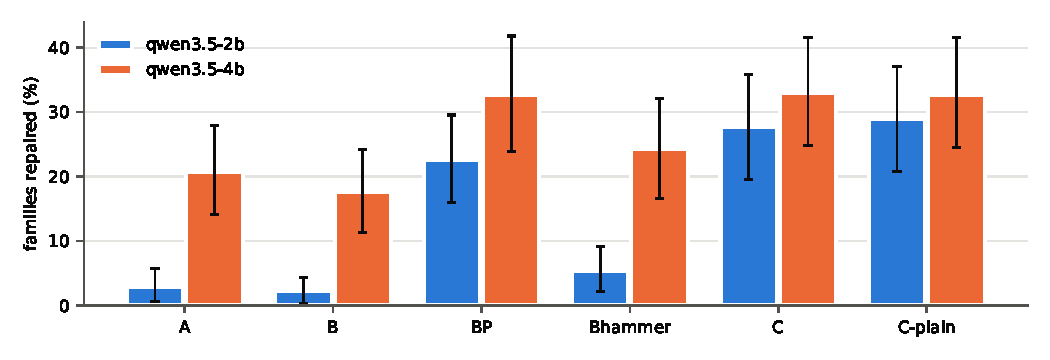
\includegraphics[width=0.9\textwidth]{fig_rates.pdf}
\caption{Verified-repair rate per condition on the \texttt{main} split, primary bug pool, as the pre-registered
family score (mean over seeds of ``any instance of the family solved''), with 95\% family-cluster bootstrap
intervals. Bhammer is exploratory.}
\label{fig:rates}
\end{figure*}}{}

% Generated by make_results.py. Do not edit by hand.
\begin{table*}[t]\centering\small
\caption{RQ1, confirmatory: paired family-level comparisons on the \texttt{main} split, primary bug pool (natural $\cup$ mutant). One-sided sign-flip test, Holm over the four primary tests; 95\% family-cluster bootstrap CI; Cohen's $h$; families solved only by $x$ / only by $y$.}\label{tab:rq1}
\begin{tabular}{@{}llrrrlrrr@{}}\toprule
Model & Comparison & Fam. & $x$ & $y$ & Diff. (pp) [95\% CI] & $p_\text{Holm}$ & $h$ & only $x$/$y$ \\\midrule
qwen3.5-2b & C vs B & 106 & 27.7\% & 2.2\% & +25.5 [+18.2, +33.0] & $<0.001$ & 0.81 & 28/0 \\
qwen3.5-2b & C vs BP & 106 & 27.7\% & 22.6\% & +5.0 [+1.6, +8.8] & 0.012 & 0.12 & 10/2 \\
qwen3.5-4b & C vs B & 106 & 33.0\% & 17.6\% & +15.4 [+9.4, +21.7] & $<0.001$ & 0.36 & 19/1 \\
qwen3.5-4b & C vs BP & 106 & 33.0\% & 32.7\% & +0.3 [$-$2.8, +3.5] & 0.500 & 0.01 & 3/2 \\
\bottomrule\end{tabular}
\end{table*}

\begin{table*}[t]\centering\small
\caption{Verified-repair rate per run on the \texttt{main} split (runs in brackets).}\label{tab:rates}
\begin{tabular}{@{}lrrrrrrrr@{}}\toprule
Model & A & B & BP & Bhammer & C & C-plain & S & S-plain \\\midrule
gemma-4-e4b-it &  & 0.9\%\,\scriptsize(231) & 22.9\%\,\scriptsize(231) &  & 25.1\%\,\scriptsize(231) &  &  &  \\
goedel-code-prover-8b & 16.5\%\,\scriptsize(231) & 20.8\%\,\scriptsize(231) &  &  &  &  &  &  \\
qwen3.5-2b & 1.9\%\,\scriptsize(693) & 1.0\%\,\scriptsize(693) & 15.9\%\,\scriptsize(693) & 3.0\%\,\scriptsize(693) & 21.6\%\,\scriptsize(693) & 22.1\%\,\scriptsize(693) & 3.7\%\,\scriptsize(267) & 4.1\%\,\scriptsize(267) \\
qwen3.5-4b & 14.4\%\,\scriptsize(693) & 11.4\%\,\scriptsize(693) & 26.3\%\,\scriptsize(693) & 18.9\%\,\scriptsize(693) & 27.6\%\,\scriptsize(693) & 27.1\%\,\scriptsize(693) & 12.7\%\,\scriptsize(267) & 12.7\%\,\scriptsize(267) \\
\bottomrule\end{tabular}
\end{table*}

\begin{table*}[t]\centering\small
\caption{Secondary and exploratory comparisons on \texttt{main} (uncorrected one-sided $p$). Never pooled with the primary estimates.}\label{tab:secondary}
\begin{tabular}{@{}llrrrlrrr@{}}\toprule
Model & Comparison & Fam. & $x$ & $y$ & Diff. (pp) [95\% CI] & $p$ & $h$ & only $x$/$y$ \\\midrule
gemma-4-e4b-it & C vs B & 106 & 30.2\% & 1.9\% & +28.3 [+19.8, +36.8] & $<0.001$ & 0.89 & 30/0 \\
gemma-4-e4b-it & C vs BP & 106 & 30.2\% & 27.4\% & +2.8 [$-$3.8, +9.4] & 0.291 & 0.06 & 8/5 \\
gemma-4-e4b-it & BP vs B & 106 & 27.4\% & 1.9\% & +25.5 [+17.9, +34.0] & $<0.001$ & 0.83 & 27/0 \\
gemma-4-e4b-it & C vs B\_noauto & 106 & 30.2\% & 0.0\% & +30.2 [+21.7, +38.7] & $<0.001$ & 1.16 & 32/0 \\
qwen3.5-2b & C vs C-plain & 106 & 27.7\% & 28.9\% & $-$1.3 [$-$3.8, +1.3] & 0.893 & -0.03 & 3/3 \\
qwen3.5-2b & C vs A & 106 & 27.7\% & 2.8\% & +24.8 [+17.6, +32.4] & $<0.001$ & 0.77 & 28/0 \\
qwen3.5-2b & BP vs B & 106 & 22.6\% & 2.2\% & +20.4 [+14.2, +27.4] & $<0.001$ & 0.69 & 20/0 \\
qwen3.5-2b & C vs B\_noauto & 106 & 27.7\% & 0.9\% & +26.7 [+19.2, +34.6] & $<0.001$ & 0.91 & 30/0 \\
qwen3.5-2b & C vs Bhammer & 106 & 27.7\% & 5.3\% & +22.3 [+15.7, +29.2] & $<0.001$ & 0.64 & 27/0 \\
qwen3.5-2b & Bhammer vs B & 106 & 5.3\% & 2.2\% & +3.1 [0.0, +6.6] & 0.057 & 0.17 & 3/2 \\
qwen3.5-2b & S vs S-plain & 89 & 3.7\% & 4.1\% & $-$0.4 [$-$2.2, +1.1] & 0.812 & -0.02 & 0/1 \\
qwen3.5-4b & C vs C-plain & 106 & 33.0\% & 32.7\% & +0.3 [$-$2.2, +2.8] & 0.500 & 0.01 & 2/1 \\
qwen3.5-4b & C vs A & 106 & 33.0\% & 20.8\% & +12.3 [+6.6, +18.2] & $<0.001$ & 0.28 & 16/1 \\
qwen3.5-4b & BP vs B & 106 & 32.7\% & 17.6\% & +15.1 [+9.4, +21.4] & $<0.001$ & 0.35 & 18/1 \\
qwen3.5-4b & C vs B\_noauto & 106 & 33.0\% & 12.3\% & +20.8 [+14.2, +27.7] & $<0.001$ & 0.51 & 24/1 \\
qwen3.5-4b & C vs Bhammer & 106 & 33.0\% & 24.2\% & +8.8 [+3.5, +14.2] & $<0.001$ & 0.20 & 12/2 \\
qwen3.5-4b & Bhammer vs B & 106 & 24.2\% & 17.6\% & +6.6 [+1.3, +11.9] & 0.011 & 0.16 & 11/3 \\
qwen3.5-4b & S vs S-plain & 89 & 12.7\% & 12.7\% & 0.0 [$-$2.6, +3.0] & 0.602 & 0.00 & 2/0 \\
\bottomrule\end{tabular}
\end{table*}

\begin{table*}[t]\centering\small
\caption{Outcome labels per run on \texttt{main}.}\label{tab:outcomes}
\begin{tabular}{@{}llrrrrr@{}}\toprule
Model & Cond. & verified repair & correct unverified & integrity violation & unresolved & runs \\\midrule
gemma-4-e4b-it & B & 2 & 88 & 103 & 38 & 231 \\
gemma-4-e4b-it & BP & 53 & 49 & 89 & 40 & 231 \\
gemma-4-e4b-it & C & 58 & 68 & 19 & 86 & 231 \\
goedel-code-prover-8b & A & 38 & 42 & 149 & 2 & 231 \\
goedel-code-prover-8b & B & 48 & 71 & 97 & 15 & 231 \\
qwen3.5-2b & A & 13 & 34 & 621 & 25 & 693 \\
qwen3.5-2b & B & 7 & 117 & 352 & 217 & 693 \\
qwen3.5-2b & BP & 110 & 55 & 312 & 216 & 693 \\
qwen3.5-2b & Bhammer & 21 & 175 & 267 & 230 & 693 \\
qwen3.5-2b & C & 150 & 86 & 168 & 289 & 693 \\
qwen3.5-2b & C-plain & 153 & 87 & 162 & 291 & 693 \\
qwen3.5-2b & S & 10 & 52 & 137 & 68 & 267 \\
qwen3.5-2b & S-plain & 11 & 53 & 129 & 74 & 267 \\
qwen3.5-4b & A & 100 & 156 & 395 & 42 & 693 \\
qwen3.5-4b & B & 79 & 132 & 408 & 74 & 693 \\
qwen3.5-4b & BP & 182 & 74 & 381 & 56 & 693 \\
qwen3.5-4b & Bhammer & 131 & 143 & 340 & 79 & 693 \\
qwen3.5-4b & C & 191 & 113 & 253 & 136 & 693 \\
qwen3.5-4b & C-plain & 188 & 135 & 215 & 155 & 693 \\
qwen3.5-4b & S & 34 & 45 & 116 & 72 & 267 \\
qwen3.5-4b & S-plain & 34 & 52 & 88 & 93 & 267 \\
\bottomrule\end{tabular}
\end{table*}

\begin{table*}[t]\centering\small
\caption{RQ5 energy on \texttt{main} (estimate, deviation D-4). GPU: tokens used $\times$ joules per token calibrated on our slice for each model (marginal board power over idle; range over three calibration cycles). CPU: Lean seconds $\times$ 5.47\,W per thread. CO$_2$ at 0.716\,kg/kWh.}\label{tab:energy}
\begin{tabular}{@{}llrrrrr@{}}\toprule
Model & Cond. & Repairs & GPU kJ & CPU kJ & kJ per repair [range] & g CO$_2$ per repair \\\midrule
gemma-4-e4b-it & B & 2 & 459 & 6 & 232.4 \scriptsize[223.1, 243.6] & 46.21 \\
gemma-4-e4b-it & BP & 53 & 400 & 65 & 8.8 \scriptsize[8.5, 9.1] & 1.75 \\
gemma-4-e4b-it & C & 58 & 118 & 33 & 2.6 \scriptsize[2.5, 2.7] & 0.52 \\
goedel-code-prover-8b & A & 38 & 409 & 3 & 10.8 \scriptsize[9.5, 12.0] & 2.15 \\
goedel-code-prover-8b & B & 48 & 404 & 5 & 8.5 \scriptsize[7.6, 9.4] & 1.69 \\
qwen3.5-2b & A & 13 & 287 & 23 & 23.9 \scriptsize[22.2, 24.9] & 4.74 \\
qwen3.5-2b & B & 7 & 355 & 35 & 55.7 \scriptsize[51.7, 58.2] & 11.08 \\
qwen3.5-2b & BP & 110 & 339 & 57 & 3.6 \scriptsize[3.4, 3.7] & 0.71 \\
qwen3.5-2b & Bhammer & 21 & 411 & 30 & 21.0 \scriptsize[19.4, 22.0] & 4.18 \\
qwen3.5-2b & C & 150 & 226 & 68 & 2.0 \scriptsize[1.8, 2.0] & 0.39 \\
qwen3.5-2b & C-plain & 153 & 247 & 63 & 2.0 \scriptsize[1.9, 2.1] & 0.40 \\
qwen3.5-2b & S & 10 & 114 & 50 & 16.3 \scriptsize[15.4, 16.9] & 3.25 \\
qwen3.5-2b & S-plain & 11 & 115 & 43 & 14.4 \scriptsize[13.6, 14.9] & 2.86 \\
qwen3.5-4b & A & 100 & 877 & 17 & 8.9 \scriptsize[7.8, 10.0] & 1.78 \\
qwen3.5-4b & B & 79 & 1039 & 23 & 13.4 \scriptsize[11.8, 14.9] & 2.67 \\
qwen3.5-4b & BP & 182 & 985 & 94 & 5.9 \scriptsize[5.3, 6.5] & 1.18 \\
qwen3.5-4b & Bhammer & 131 & 814 & 30 & 6.4 \scriptsize[5.7, 7.1] & 1.28 \\
qwen3.5-4b & C & 191 & 430 & 69 & 2.6 \scriptsize[2.4, 2.9] & 0.52 \\
qwen3.5-4b & C-plain & 188 & 373 & 65 & 2.3 \scriptsize[2.1, 2.5] & 0.46 \\
qwen3.5-4b & S & 34 & 238 & 29 & 7.9 \scriptsize[7.0, 8.6] & 1.56 \\
qwen3.5-4b & S-plain & 34 & 201 & 33 & 6.9 \scriptsize[6.2, 7.5] & 1.37 \\
\bottomrule\end{tabular}
\end{table*}

\begin{table*}[t]\centering\small
\caption{Held-out replication (analysed once and separately; not confirmatory).}\label{tab:heldout}
\begin{tabular}{@{}llrrrlrrr@{}}\toprule
Model & Comparison & Fam. & $x$ & $y$ & Diff. (pp) [95\% CI] & $p_\text{Holm}$ & $h$ & only $x$/$y$ \\\midrule
qwen3.5-2b & C vs B & 46 & 20.3\% & 1.4\% & +18.8 [+9.4, +29.0] & $<0.001$ & 0.69 & 10/0 \\
qwen3.5-2b & C vs BP & 46 & 20.3\% & 20.3\% & 0.0 [$-$4.3, +4.3] & 1.000 & 0.00 & 2/1 \\
qwen3.5-4b & C vs B & 46 & 29.7\% & 10.1\% & +19.6 [+10.1, +30.4] & $<0.001$ & 0.50 & 11/0 \\
qwen3.5-4b & C vs BP & 46 & 29.7\% & 29.7\% & 0.0 [$-$4.3, +5.8] & 1.000 & 0.00 & 1/0 \\
\bottomrule\end{tabular}
\end{table*}

\begin{table*}[t]\centering\small
\caption{Pilot (calibration split: 20 families, 41 buggy instances, seed 11; per-run rate, runs in brackets). Never pooled with the study.}\label{tab:pilotirel}
\begin{tabular}{@{}lrrrrrr@{}}\toprule
Model & A & B & BP & Bhammer & C & C-plain \\\midrule
qwen3.5-2b & 0.0\%\,\scriptsize(41) & 0.0\%\,\scriptsize(41) & 12.2\%\,\scriptsize(41) & 2.4\%\,\scriptsize(41) & 26.8\%\,\scriptsize(41) & 19.5\%\,\scriptsize(41) \\
qwen3.5-4b & 22.0\%\,\scriptsize(41) & 19.5\%\,\scriptsize(41) & 31.7\%\,\scriptsize(41) & 22.0\%\,\scriptsize(41) & 36.6\%\,\scriptsize(41) & 26.8\%\,\scriptsize(41) \\
\bottomrule\end{tabular}
\end{table*}


\subsection{RQ2: shaping, reverting and study S}
\resRQTwoText

\subsection{RQ3: structured hint vs plain retry}
\resRQThreeText

\subsection{RQ4: which code shapes automation proves}
\resRQFourText

\subsection{RQ5: costs, scale and the proof specialist}
\IfFileExists{fig_costs.pdf}{%
\begin{figure}[t]\centering
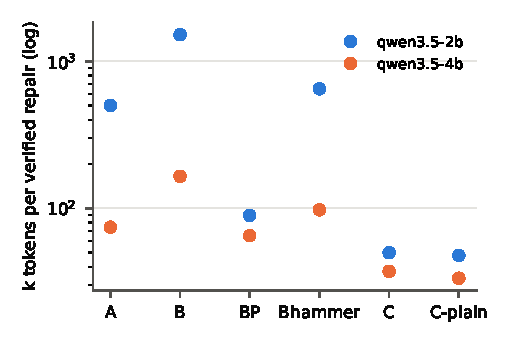
\includegraphics[width=\columnwidth]{fig_costs.pdf}
\caption{Model tokens spent per verified repair (log scale), \texttt{main} split, primary models. Missing points
mean no verified repair in that cell.}
\label{fig:costs}
\end{figure}}{}
\resRQFiveText

\subsection{Secondary: B without automation, Bhammer and cross-evaluation}
\resSecondaryText

\subsection{Held-out replication}
\resHeldoutText

\section{Threats to Validity}
\textbf{Construct.} A proof certifies only its specification. Every verified repair must also pass hidden tests,
and ``verified but behaviourally wrong'' is reported separately as a weak-contract signal. Known-defective tasks
are excluded.
\textbf{Selection.} Portfolio coverage is reported over the full eligible pool; condition T is a screening and
stratification variable only, never a filter on tasks.
\textbf{Hand-tuning.} Prompts, portfolio and hints were tuned on pilot families only, then frozen; the held-out
split was run once.
\textbf{Specification gaming.} Static rejection, the axiom check, degeneracy flags and a 10\% stratified hand
audit plus every flagged success guard against it.
\textbf{Internal.} Budgets and turn-0 information are equal; BP gives B the same automation first, Bhammer tells
B the automation, B\_noauto and the cross-evaluation test whether B is a strawman.
\textbf{Statistical.} C vs BP is underpowered by the fixed size of VERINA (\cref{tab:power}); a tie there is
reported as such, with cost per repair.
\textbf{External.} VERINA functions are small; results are for 4-bit models and two model families, on one GPU
model, and may not transfer to full precision or to repository-scale Lean.
\textbf{Hardware.} Every step used one GPU slice, one host and one llama.cpp build, so no comparison mixes
environments. The slice ran no job beyond our two study lanes. The physical GPU hosts other users' slices, which
would have made per-condition energy unattributable even with a correct counter (deviation D-1); verdicts do not
depend on it. The pilot is a calibration on its own
split and is never pooled with the study.

\section{Conclusion}
\resConclusionText

\paragraph{Artefacts.} The harness, buggy-VERINA dataset with hidden tests, frozen configuration, deviation log
and all run logs are in the Leanstein repository.

\FloatBarrier
\bibliographystyle{plain}
\bibliography{refs}
\end{document}
